\documentclass{standalone}
\usepackage{tikz}
\usetikzlibrary{patterns, positioning}
\usepackage[sfdefault]{ClearSans} %% option 'sfdefault' activates Clear Sans as the default text font
\usepackage[T1]{fontenc}

\begin{document}
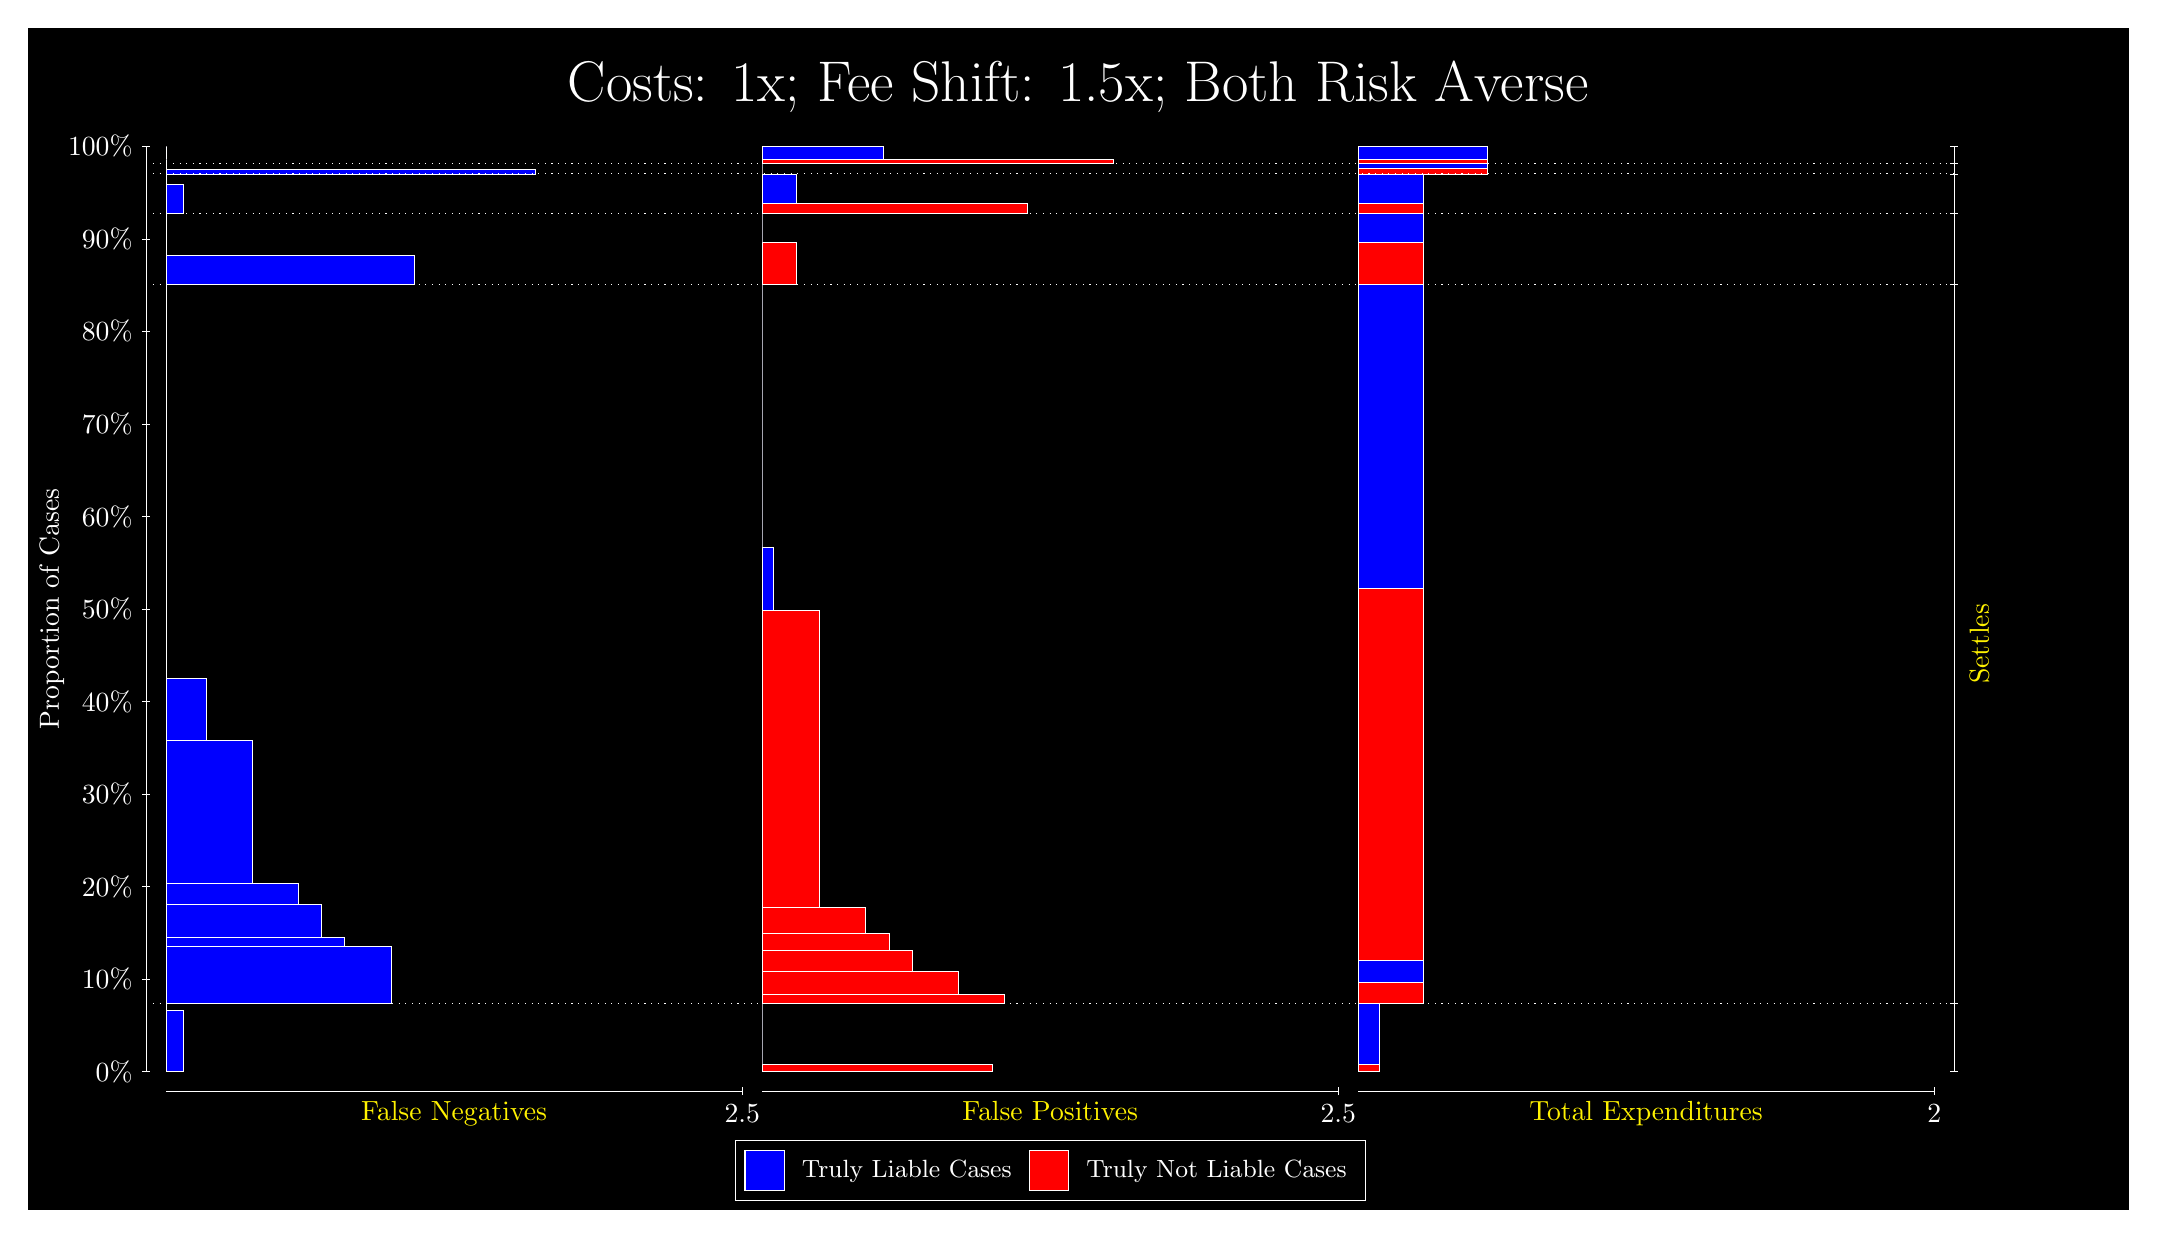
\begin{tikzpicture}
\draw[fill=black] (0,0) rectangle (26.667,15);
\draw[text=white] (0,13.5) rectangle (26.667,15) node[midway] {\huge Costs: 1x; Fee Shift: 1.5x; Both Risk Averse};
\draw[white, very thin] (1.5,1.75) -- (1.5,13.5);
\node[rotate=90, text=white, anchor=center] at (0.3, 7.625) {Proportion of Cases};
\draw[white, very thin] (1.45,1.75) -- (1.55,1.75);
\node[text=white, anchor=east] at (1.45, 1.75) {0\%};
\draw[white, very thin] (1.45,2.925) -- (1.55,2.925);
\node[text=white, anchor=east] at (1.45, 2.925) {10\%};
\draw[white, very thin] (1.45,4.1) -- (1.55,4.1);
\node[text=white, anchor=east] at (1.45, 4.1) {20\%};
\draw[white, very thin] (1.45,5.275) -- (1.55,5.275);
\node[text=white, anchor=east] at (1.45, 5.275) {30\%};
\draw[white, very thin] (1.45,6.45) -- (1.55,6.45);
\node[text=white, anchor=east] at (1.45, 6.45) {40\%};
\draw[white, very thin] (1.45,7.625) -- (1.55,7.625);
\node[text=white, anchor=east] at (1.45, 7.625) {50\%};
\draw[white, very thin] (1.45,8.8) -- (1.55,8.8);
\node[text=white, anchor=east] at (1.45, 8.8) {60\%};
\draw[white, very thin] (1.45,9.975) -- (1.55,9.975);
\node[text=white, anchor=east] at (1.45, 9.975) {70\%};
\draw[white, very thin] (1.45,11.15) -- (1.55,11.15);
\node[text=white, anchor=east] at (1.45, 11.15) {80\%};
\draw[white, very thin] (1.45,12.325) -- (1.55,12.325);
\node[text=white, anchor=east] at (1.45, 12.325) {90\%};
\draw[white, very thin] (1.45,13.5) -- (1.55,13.5);
\node[text=white, anchor=east] at (1.45, 13.5) {100\%};

\draw[white, very thin] (24.457,1.75) -- (24.457,13.5);
\draw[white, very thin] (24.407,1.75) -- (24.507,1.75);
\node[anchor=west] at (24.407, 1.75) {};
\draw[white, very thin] (24.407,2.6182) -- (24.507,2.6182);
\node[anchor=west] at (24.407, 2.6182) {};
\draw[white, very thin] (24.407,11.745) -- (24.507,11.745);
\node[anchor=west] at (24.407, 11.745) {};
\draw[white, very thin] (24.407,12.649) -- (24.507,12.649);
\node[anchor=west] at (24.407, 12.649) {};
\draw[white, very thin] (24.407,13.15) -- (24.507,13.15);
\node[anchor=west] at (24.407, 13.15) {};
\draw[white, very thin] (24.407,13.28) -- (24.507,13.28);
\node[anchor=west] at (24.407, 13.28) {};
\draw[white, very thin] (24.407,13.5) -- (24.507,13.5);
\node[anchor=west] at (24.407, 13.5) {};

\draw[white, very thin, fill=blue] (1.75,1.75) rectangle (1.9696,2.5269);
\draw[white, very thin, fill=red] (1.75,2.5269) rectangle (1.75,2.6182);
\draw[white, very thin, fill=blue] (1.75,2.6182) rectangle (4.6044,3.3455);
\draw[white, very thin, fill=blue] (1.75,3.3455) rectangle (4.0188,3.4591);
\draw[white, very thin, fill=blue] (1.75,3.4591) rectangle (3.7261,3.8727);
\draw[white, very thin, fill=blue] (1.75,3.8727) rectangle (3.4333,4.1469);
\draw[white, very thin, fill=blue] (1.75,4.1469) rectangle (2.8478,5.9567);
\draw[white, very thin, fill=blue] (1.75,5.9567) rectangle (2.2623,6.7488);
\draw[white, very thin, fill=red] (1.75,6.7488) rectangle (1.75,11.745);
\draw[white, very thin, fill=blue] (1.75,11.745) rectangle (4.8971,12.118);
\draw[white, very thin, fill=red] (1.75,12.118) rectangle (1.75,12.649);
\draw[white, very thin, fill=blue] (1.75,12.649) rectangle (1.9696,13.024);
\draw[white, very thin, fill=red] (1.75,13.024) rectangle (1.75,13.15);
\draw[white, very thin, fill=blue] (1.75,13.15) rectangle (6.4341,13.204);
\draw[white, very thin, fill=red] (1.75,13.204) rectangle (1.75,13.28);
\draw[white, very thin, fill=red] (1.75,13.28) rectangle (1.75,13.335);
\draw[white, very thin, fill=blue] (1.75,13.335) rectangle (1.75,13.5);
\draw[white, very thin, fill=red] (9.3189,1.75) rectangle (12.246,1.8413);
\draw[white, very thin, fill=blue] (9.3189,1.8413) rectangle (9.3189,2.6182);
\draw[white, very thin, fill=red] (9.3189,2.6182) rectangle (12.393,2.7291);
\draw[white, very thin, fill=red] (9.3189,2.7291) rectangle (11.807,3.0197);
\draw[white, very thin, fill=red] (9.3189,3.0197) rectangle (11.222,3.2895);
\draw[white, very thin, fill=red] (9.3189,3.2895) rectangle (10.929,3.5061);
\draw[white, very thin, fill=red] (9.3189,3.5061) rectangle (10.636,3.83);
\draw[white, very thin, fill=red] (9.3189,3.83) rectangle (10.051,7.6142);
\draw[white, very thin, fill=blue] (9.3189,7.6142) rectangle (9.4652,8.4063);
\draw[white, very thin, fill=blue] (9.3189,8.4063) rectangle (9.3189,11.745);
\draw[white, very thin, fill=red] (9.3189,11.745) rectangle (9.758,12.276);
\draw[white, very thin, fill=blue] (9.3189,12.276) rectangle (9.3189,12.649);
\draw[white, very thin, fill=red] (9.3189,12.649) rectangle (12.686,12.775);
\draw[white, very thin, fill=blue] (9.3189,12.775) rectangle (9.758,13.15);
\draw[white, very thin, fill=red] (9.3189,13.15) rectangle (9.3189,13.226);
\draw[white, very thin, fill=blue] (9.3189,13.226) rectangle (9.3189,13.28);
\draw[white, very thin, fill=red] (9.3189,13.28) rectangle (13.783,13.335);
\draw[white, very thin, fill=blue] (9.3189,13.335) rectangle (10.856,13.5);
\draw[white, very thin, fill=red] (16.888,1.75) rectangle (17.162,1.8413);
\draw[white, very thin, fill=blue] (16.888,1.8413) rectangle (17.162,2.6182);
\draw[white, very thin, fill=red] (16.888,2.6182) rectangle (17.711,2.8881);
\draw[white, very thin, fill=blue] (16.888,2.8881) rectangle (17.711,3.1623);
\draw[white, very thin, fill=red] (16.888,3.1623) rectangle (17.711,7.8884);
\draw[white, very thin, fill=blue] (16.888,7.8884) rectangle (17.711,11.745);
\draw[white, very thin, fill=red] (16.888,11.745) rectangle (17.711,12.276);
\draw[white, very thin, fill=blue] (16.888,12.276) rectangle (17.711,12.649);
\draw[white, very thin, fill=red] (16.888,12.649) rectangle (17.711,12.775);
\draw[white, very thin, fill=blue] (16.888,12.775) rectangle (17.711,13.15);
\draw[white, very thin, fill=red] (16.888,13.15) rectangle (18.534,13.226);
\draw[white, very thin, fill=blue] (16.888,13.226) rectangle (18.534,13.28);
\draw[white, very thin, fill=red] (16.888,13.28) rectangle (18.534,13.335);
\draw[white, very thin, fill=blue] (16.888,13.335) rectangle (18.534,13.5);
\draw[white, dotted] (1.5,2.6182) -- (24.457,2.6182);
\draw[white, dotted] (1.5,11.745) -- (24.457,11.745);
\draw[white, dotted] (1.5,12.649) -- (24.457,12.649);
\draw[white, dotted] (1.5,13.15) -- (24.457,13.15);
\draw[white, dotted] (1.5,13.28) -- (24.457,13.28);
\draw[white, very thin] (1.75,1.5) -- (9.0689,1.5);
\node[text=yellow, anchor=north] at (5.4094, 1.5) {False Negatives};
\draw[white, very thin] (9.0689,1.45) -- (9.0689,1.55);
\node[text=white, anchor=north] at (9.0689, 1.45) {2.5};

\draw[white, very thin] (9.3189,1.5) -- (16.638,1.5);
\node[text=yellow, anchor=north] at (12.978, 1.5) {False Positives};
\draw[white, very thin] (16.638,1.45) -- (16.638,1.55);
\node[text=white, anchor=north] at (16.638, 1.45) {2.5};

\draw[white, very thin] (16.888,1.5) -- (24.207,1.5);
\node[text=yellow, anchor=north] at (20.547, 1.5) {Total Expenditures};
\draw[white, very thin] (24.207,1.45) -- (24.207,1.55);
\node[text=white, anchor=north] at (24.207, 1.45) {2};


\node[text=yellow, centered, rotate=90] at (24.777, 7.1815) {Settles};





\draw (12.978300999999998,1.5) node[draw=none] (baseCoordinate) {};
\begin{scope}[align=center]
        \matrix[scale=0.5, draw=white, below=0.5cm of baseCoordinate, nodes={draw}, column sep=0.1cm]{
            \node[rectangle, draw, minimum width=0.5cm, minimum height=0.5cm, fill=blue] {}; &
            \node[draw=none, font=\small, text=white] (B) {Truly Liable Cases}; &
            \node[rectangle, draw, minimum width=0.5cm, minimum height=0.5cm, fill=red] {}; &
            \node[draw=none, font=\small, text=white] (B) {Truly Not Liable Cases}; \\
            };
\end{scope}

\end{tikzpicture}
\end{document}